\documentclass[sigconf]{acmart}

\usepackage{booktabs} % For formal tables
\usepackage{multirow}

% Copyright
\setcopyright{none}
%\setcopyright{acmcopyright}
%\setcopyright{acmlicensed}
% \setcopyright{rightsretained}
%\setcopyright{usgov}
%\setcopyright{usgovmixed}
%\setcopyright{cagov}
%\setcopyright{cagovmixed}

\begin{document}


\title{Logical Data Deduplication For Backup}

% \author{Lars Th{\o}rv{\"a}ld}
% \authornote{This author is the
%   one who did all the really hard work.}
% \affiliation{%
%   \institution{The Th{\o}rv{\"a}ld Group}
%   \streetaddress{1 Th{\o}rv{\"a}ld Circle}
%   \city{Hekla} 
%   \country{Iceland}}
% \email{larst@affiliation.org}




\begin{abstract}

Security plays a vital role when people deploy services in the cloud,so encryption is ofthen used. Computing over encrypted data has prove useful in such situation. Cryptdb\citep{popa2011cryptdb} is such kind of system. To support more operation on encrypted data, Cryptdb uses the multi-onion design, which produce significant storage overhead when we need to backup the data. Traditional data deduplication technique do not work well on encrypted data. In this paper, we1 present the chanllenges we meet when we need to backup data using popular data backup tools, and we propose a new backup method with the help of metadata and implement a new tool Cryptdump for cryptedb. Experiments show that our method can  significantly reduce the storage size with little overhead. Our deduplication method can also be used together with traditional data deduplication methods to further reduce the storage size.








\end{abstract}



\maketitle

\section{Introduction}

Services on cloud today subject to much more threats than ever. Users' private data on cloud could be unauthorized accessed by hackers or their adversaries in various ways.
With the development of cloud computing, more services are deployed in the cloud. Security is the first issue to taken into consideration when people store their data in the cloud. Encryption is an important technique to ensure data security. However, for a database system, when data is encrypted, it could be hard for people to perform operations on those data. Fortunately, with the help of certain encryption schemes, computing over encrypted data is possible. CryptDB\citep{popa2011cryptdb}, which was proposed in sosp'11, is such kind of system. Similarity system has been implemented by many companies like google,SAP,Microsoft,and some Startups\citep{cryptdbsite} \citep{kerschbaum2013encrypted}.


The idea of computing over encrypted data came from homomorphic encryption. Fully Homomorphic encryption is too expensive\citep{gentry2009fully}, however, to support common database operation, fully homomorphic is not the only way. The main idea of Cryptdb is to use the characteristics of several encryption schemes to support different operations on columns in a relational table.  Since each encryption scheme can only support one operation, to allow multiple operations, each column in the table is duplicated many times according to how many operations each column need to support, and different encryption schemes are applied to each copy. Such data layout allows computing over encrypted data, but incur huge storage overhead at the same time. According to the author\citep{popa2011cryptdb}, experiments with TPC-C showed an increase of 3.76 times of storage size.

Another import issue of a cloud database system is data integrity. The system may suffer from disk failures or system crash, so database backup is needed for such systems. In fact, operators of a database system may come across problems like Operating system crash, power failure, file system crash or Hardware problem\citep{mysqlbackupdocumentation}.


This storage overhead is inevitable when we want to support different operations. However, for a data backup, this duplication is unnecessary since we do not perform operations on the backup.

To reduce storage overhead in backup, data deduplication techniques are often used. In fact, data deduplication has become a standard component for backup systems\citep{fu2015design}. However, for cryptdb, traditional deduplication methods are limited since it could be hard to deduplicate encrypted data, and those methods are unaware of the relations between encrypted data. There are research about deduplicating encrypted data, but they focus on user files in the cloud instead of database systems. 

Cryptedb records how the original tables are encrypted and how the columns are replicated. We call those data metadata in this paper. It stores metadata on the proxy. If we introduce this kind of extra information, data deduplication for backup system can be more efficient. And also, the onion layout of fields allow us to make tradeoff between storage size, recover time, and data security.


In this paper, we raise the question that how can we reduce the the overhead of storage with the help of metadata, and that how to use the information to make proper tradeoff. We should consider storage size, security and the time consumed for data recovery. In our work, we propose a new data deduplication method for Cryptdb, which utilizes metadata information to help find duplicates in encrypted data. We implemented a tool called Cryptdbdump and did experiments with TPC-C-MySQL in the newest version of Cryptdb.


To realise this, we need to address three main challenges:

1) How to parse the metadata of Cryptdb

2) How  does the time and space overhead change as the onions and layers change

3) How to choose the right onion and layer to make optimal backup


To tackle those problems, we need to

1) analyse the structure of metadata in Cryptdb and find duplicates

2) do analysis on different onions and layers of encryption scheme and provide statiscis

3) design a strategy for data backup with the help of metadata and the costs information 

To summarize, we make the following contributions.

1) A full analysis of the cost of each layer and onion in Cryptdb

2) A new data deduplication method for Cryptdb that utilizes metadata information 

3) A strategy for choosing the right portion of data for backup, which taken storage size, 

4) An implementation of data backup tool called Cryptedbdump 

To our knowledge, we are the first to propose a deduplication method for Cryptdb with the help of metadata to reduce storage overhead, and our high level deduplication method can be used together with traditional deduplication techniques like block level comparision \citep{bellare2013message}.

The rest of this paper is structured as follows. In section 2, we introduce the structure of cryptdb and the structure of encryption metadata in the newest version of Cryptdb. Then, we introduction the characteristics of the encryption schemes use in Cryptdb in section 3. And in section 4, we introduce popular data backup and deduplication methods. In section 5, we introduce our design details and results of experiments. In section 6 we introduce related work. And Section 7 concludes the paper.
\\ \\ \\ 




\section{Introduction to Cryptdb}

This section introduces the structure of Cryptdb to show how data is duplicated. This introduction is based on the cryptdb paper\citep{popa2011cryptdb} and the newest verion of Cryptdb implementation at \citep{cryptdbsite}. We would like to introduce the following content.



\begin{itemize}
\item[--] The overall structure of cryptdb and the related system
\item[--] The logical view of a table in cryptdb
\item[--] Structure of the encryption metadata
\end{itemize}

This section intends to give you insight on how we find duplicates in Cryptdb, and important issues to consider when designing a backup system for cryptdb. Also, some important terms in cryptdb will be explain.

\subsection{Structure of Cryptdb}

In the cryptdb system, there are three components: client, server, and proxy. The Client is usually a webserver, and the server has MySQL  or other DBMS installed. In our current environment, we use MySQL5.7 as DBMS and MySQL-Proxy0.8.5 as proxy. The client communicate with the proxy instead of communicating directly with the server. The MySQL server is not trusted while the Proxy is trusted. When the client receive DDL queries, it will stored related encryption metadata to describe the encryption scheme of each table. For both DML and DDL queries, the proxy perform query rewrite to encrypt the query and send encrypted query to MySQL server. The results are sent to the proxy first for decryption, and then plain text will be sent to client. Figure~\ref{fig:stack1} shows the four steps of executing a SQL query in a system using Cryptdb and the two steps of executing SQL queries in a system using normal database system.



\begin{figure}[tb]
\centering
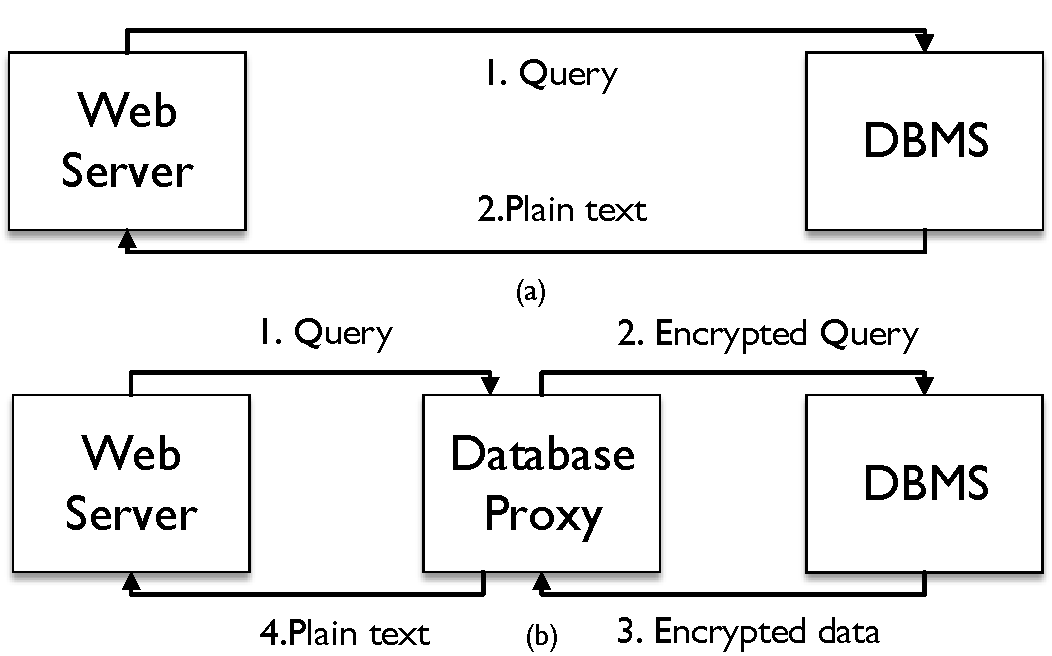
\includegraphics[width=6cm]{images/Cryptdb-structure.pdf}
\caption{structure of cryptdb}
\label{fig:stack1}
\end{figure}



\subsection{data layout and structure}

In this section, we talk about the onion encryption model and how an original plaintext table is expanded. Since there are currently only two data type supported in cryptdb, we will use an example table with those two data types: String and Integer. Figure~\ref{fig:stackx} shows how the data columns of the original plain text table are extended. For integer type, one original column is replicated for three times and encrypted using three differnt onions, the forth column IV is 64bits random integer used for encryption and decryption of the replicated columns. The column of Integer type is also replicated three times. And IV is used for the same purpose. Each of the replicated column is called an onion column. The onion is binded with several encryption layers, and each layer has it's own encryption key. The name of the onion columns indicates the onion's function: Onion DET support equal comparison; Onion OPE has the properity of order preserving; Onion Search allow searching on cipher text ; Onion HOM allow addation on ciphertext. So the queries for the web server against the columns on the original table is transformed into queries against the encrypted onion columns. If we want equal comparison, we can use the onion DET. If we need order comparison like order by, we can use the onion OPE. So different onion support different operation on the ciphertext. 




\begin{figure}[tb]
\centering
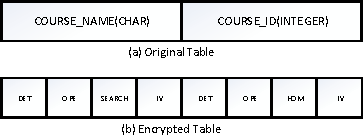
\includegraphics[width=6cm]{images/extend.pdf}
\caption{Extended table}
\label{fig:stackx}
\end{figure}

For security purposes, each onion also have two or more layers. Figure~\ref{fig:stack2}(a) provides illustration of the onions for string, and Figure~\ref{fig:stack2}(b) shows the layout of the onions for integer type. We can find that in each onion, the original plain text is encrypted several times through layers of encryption. For example, onion O-DET-STR has three layers. Suppose that the plaintext is 'p1', and it is first encrypted using AES\_CMC, and we get the ciphertext 'c1'. Then in the second layer DET\_STR, 'c1' is used as input and we still use AES\_CMC for encryption, the result is 'c2'. Finally in the RND\_STR layer, AES\_CBC is used, and we get the final result 'c3'. It should be noted that random IV is used for encryption in the RND layer. So for this O-DET-STR column, two identical values are still the same in the first two layers, However, they are different when they reach the third layer because IV is used together with encryption key for encryption in this layer. Since each row in the table has thier own random IV for each field, the ciphertext for identical plaintext may not be identical. 

Different layers of one onion provide different level of security and also different function. The layer RND is random, so it can not provide any function. The layer DET-STR allow equal comparison, and the layer DET-JOIN-STR allow equal join operation between two tables. It should be noted that the onion DET only support equal comparison operation, and no layer of this onion can support order comparison or other functions. So in summary, each onion support one kind of operation, and each level of the onion reveal different level of that ability.





\begin{figure}[tb]
\centering
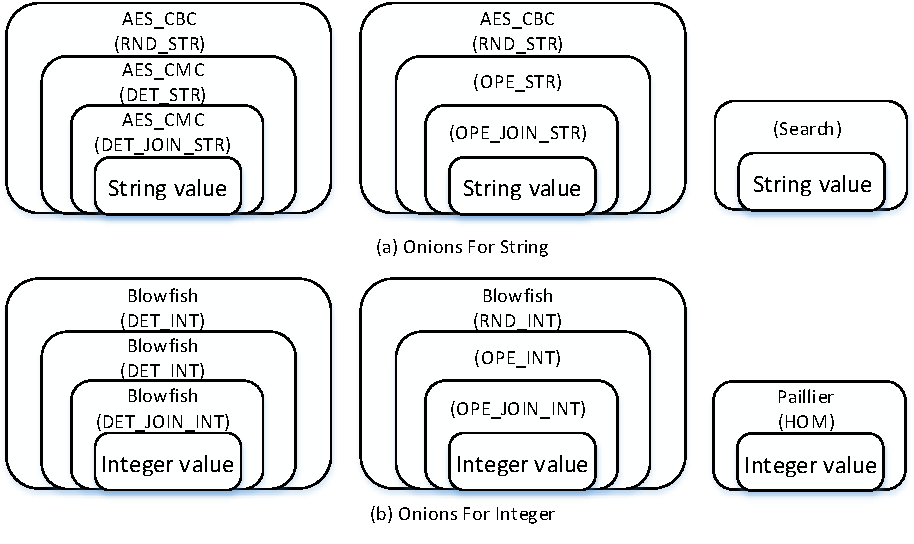
\includegraphics[width=8cm]{images/Onions.pdf}
\caption{Onion encryption layers for integer type}
\label{fig:stack2}
\end{figure}


\subsection{metadata layout and structure}

This section talks about metadata layout. Metadata is stroed in the proxy. It records the encryption details of the table in the DBMS. For example, we can read and parse the metadata to find how many databases are created. For each database, we can find how many table are in it. For each table, we can find how many fields it has, and for each field, the detailed information of the onions and layers are recorded. Those information will impact how we make choices when we bakcup data. The metadata form a hirechy from the database level to the encryption layer level. It has a structure of a tree, and is encoded and stored in a relational table. The amount of metadata is related only to the number tables and the number of fields in those tables, so the storage size is relatively small.

% Figure~\ref{fig:stack2} shows the structure of onionmeta. This is the information we need for logical deduplication. 



% \begin{figure}[tb]
% \centering
% 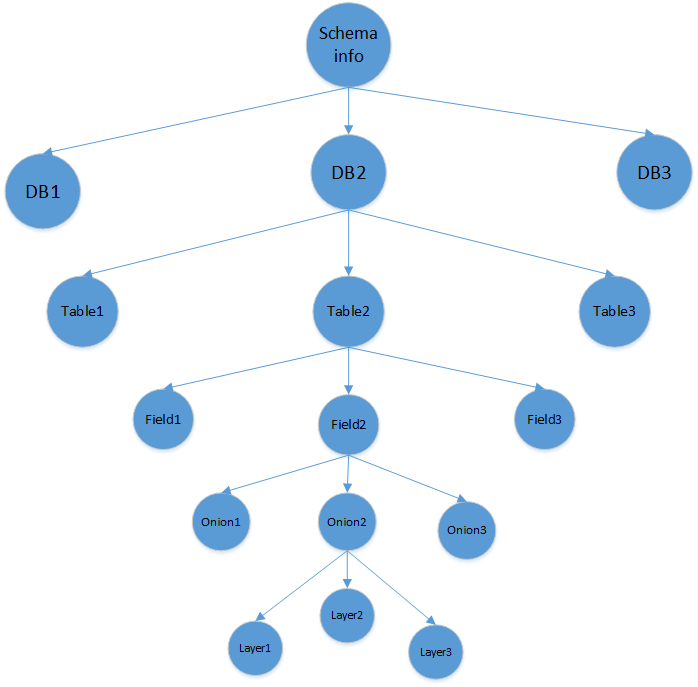
\includegraphics[width=4cm]{images/layers.png}
% \caption{Onionmeta layout}
% \label{fig:stack3}
% \end{figure}


% Every node in the tree is storaed as a record with a unique id in a relational table. The relation among nodes and the content of a node is also stored in the same table. Each onion represents an encryption scheme, which has many layers. This tree structure can be stored in a simple relational table, 

% % CREATE TABLE MetaObject(id bigint(20) unsigned auto\_increment, parent\_id bigint(20),serial\_key varbinary(500),serial\_object varbinary(500));  


% So the metadata of databases, tables, fields, onions, layers are all serialized and stored in the proxy. 

% Since the amount of data is related only to the number tables and the number of fields in those tables, the storage size is small. Also, metadata is needed for decryption and data recovery, so we use physical backup and do not deduplicate the metadata. Metadata is in the form is plaintext, so traditional deduplication techinques can work properly.


\section{Encryption schemes}


\subsection{data layers for string type}

For string type, the newest version of cryptdb only support two onions: DET and OPE. Search was removed. Also, since the onion search has only one layer and it's quit easy to do analysis, we focus on the other two layers
in this section. For onion DET, the DET layers uses 128bits AEC-CMC encryption, which is a simple wrapper function of AES-CBC. AES-CBC will pad the plaintext if the size of plaintext can not be divided by the block size. For simplicity, in the current inplementation, if the input can be diveded by the block size, the size of the datatype is expanded by one block size. So, as we add more layers to the onion, the size of the datatype keeps increasing. 

For OPE-str, the data type will be transformed to 64 bits integer. Therefore, the characteristic of OPE-str is constrained to 64bits. The for the RND layer, blowfish will be used since the data type is transformed to integer. OPE is used only for comparing and sinced it loses information, we can not decrypt ope-str. So this onion is not suitable for backup. 

Figure 3.2 provides illustration of the onions. 



\subsection{data layers for integer}

For integer type, cryptdb create three onion: DET, OPE, and HOM. Figure 3.1 shows the layout of the onions. Hom expand any type of integer to 2048 bits binarychar. For DET and OPE, the type conversion is more complex. DET layer uses blowfish encryption, which requires 64bits integer. RND for integer also uses blowfish encryption. So for DET onion, any integer will be at most expanded to 64 bits long. For onion OPE, the first layer requires that the size of cipher text is twice the size of plaintext. If the size of ciphertext is larger than 64bits thus unable to fit into an integer type, varbinary is used instead. 



\subsection{data layout and structure}

In this section, we talk about the onion layout and How an original table is expanded whith a specific onionlayout. Since the only two data type supported for encryption, we will use and imginery table with those two data types. 



\begin{figure}[tb]
\centering
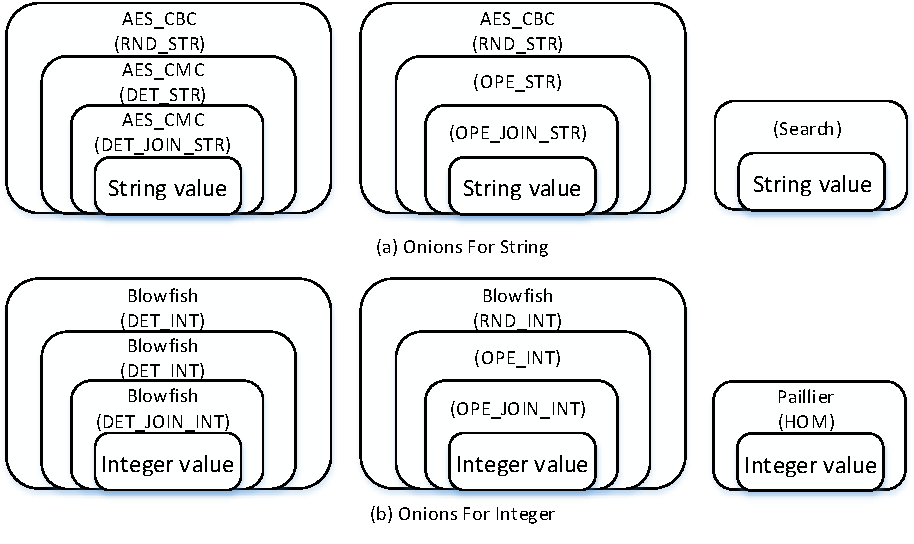
\includegraphics[width=8cm]{images/Onions.pdf}
\caption{Onion encryption layers for integer type}
\label{fig:stack3}
\end{figure}


\section{database backup methods and deduplication}

Data backup is an important functionality of database systems. All the popular database systems have backup methods. Based on how the backup is stored, we can can have two categorities of backup methods: logical backup and physical backup. Backup tools focus on low storage overhead and fast recovery. Since we do experiment with MySQL, this section focus on backup methods for MySQL. Other systems will be similar. We use backup to deal with disasters. In this section, we introduce popular backup methods. Typical backup methods also provide functions like encryption for security and compression for saving disk space.GPG tools is used for encryption.



\subsection{logical backup}

Logical backup save information in the form of SQL queries \citep{mysqlbackupdocumentatio}. For Logical backup, it's easy to control the backup granularity, and it's highly portable since the backup is in text format. MySQLdump and MySQLdumper\citep{mysqldumpper} are examples of Logical backup tools. We can also use SELECT .. INTO OUTFILE to create delimited-text files for logical backup. The basic process of logical backup is first to use select queries to pull data from the MySQL-server, and then use the data to construct Insert queries and save them into a text file. Also, Create table queries will be saved into files for recovery. We can also categorize backup method by other creterions, since we can about storage size and the logical deduplcation, we only discuss two types of backup here.





Here we describe a typical logical backup command.


\begin{itemize}
\item[--] mkdir /backups/mysqldump
\item[--] mysqldump --single-transaction --all-databases |gzip > /backups/mysqldump/today.sql.gz 
\end{itemize}






                                                 

As we can see, we can create a directory and use simple mysqldump command and options to backup our data into a file. Also, compression methods like gzip are ofthen used.

Also, If you use mydumper, you can use the following commands.

\begin{itemize}
\item[--] mkdir -p /backups/mydumper/today
\item[--] mydumper --outputdir=/backups/mydumper/today --host=localhost --compress --kill-long-queries --verbose=3 --build-empty-files --triggers --events -routines 
\end{itemize}

 
To recover the data, we can just uncompress the data and executre the sql query in the .sql file. 

you can also use binlog for backup and recovery.

\begin{itemize}
\item[--] mkdir -p /backups/binlogs
\item[--] cd /backups/binlogs
\item[--] mysqlbinlog --raw --read-from-remote-server --stop-never --verify-binlog-checksum --host=192.168.56.201 --stop-never-slave-server-id=999 mysql-bin.000001
\end{itemize}


\subsection{physical backup}

Physical bakcup consists of raw copies of directories and files that store the database contents\citep{mysqlbackupdocumentation}. In fact, simple commands like cp can be used as physical backup method. Popular physical backup tools includes ibbackup and XtraBackup\citep{xtrabackup}. MySQL store data in a set of files in a directory. Typical files includes .
This type of backup is fast since they do not convert data into logical form. Since the metadata show the data in logical form, we choose to design our strategy based on logical backup. 


Here we describe a typical physical backup workflow. 

(to be added)

The recovery form physical backup is easy. Just to uncompress the backup files and then move it the the mysql directory. 


\begin{itemize}
\item[--] service mysql stop
\item[--] rm -rf /data/mysql
\item[--] cd /backups/mylvmbackup
\item[--] tar zxf <backup file>
\item[--] mv backup/mysql /data/mysql
\item[--] service mysql start
\end{itemize}


We can find that logical backup allow user to find duplicate in the database directly, so in our design, we give our design based on logical backup.


\section{Our Analysis}

In this section, we will analyze the details of each onion design. As we stated before, Based on those analysis, we propose backup strategies for each data type accordingly. Intuitively, the strategy is to the find the smallest onion to backup and recover. In this discussion, we will focus on backup for each column, and the situation for a table should be the same. 
% The onion 'search' for string is not yet implemented in the newest version of CryptDB, so for this onion, our analysis is based on the description in \citep{song2000practical}.

In CryptDB, each column in a table can be encrypted into several onions. Each onion can have several layers. We have to make a choice whether to remove or retain a onion. If one column has three onions, we will have eight choices. Since we can not remove all of the onions, there are seven possible choices. For each onion, we can either choose to backup it directly, or to decrypt some layers and then backup it. We will discuss whether those choices are practical.

\begin{figure}[tb]
\centering
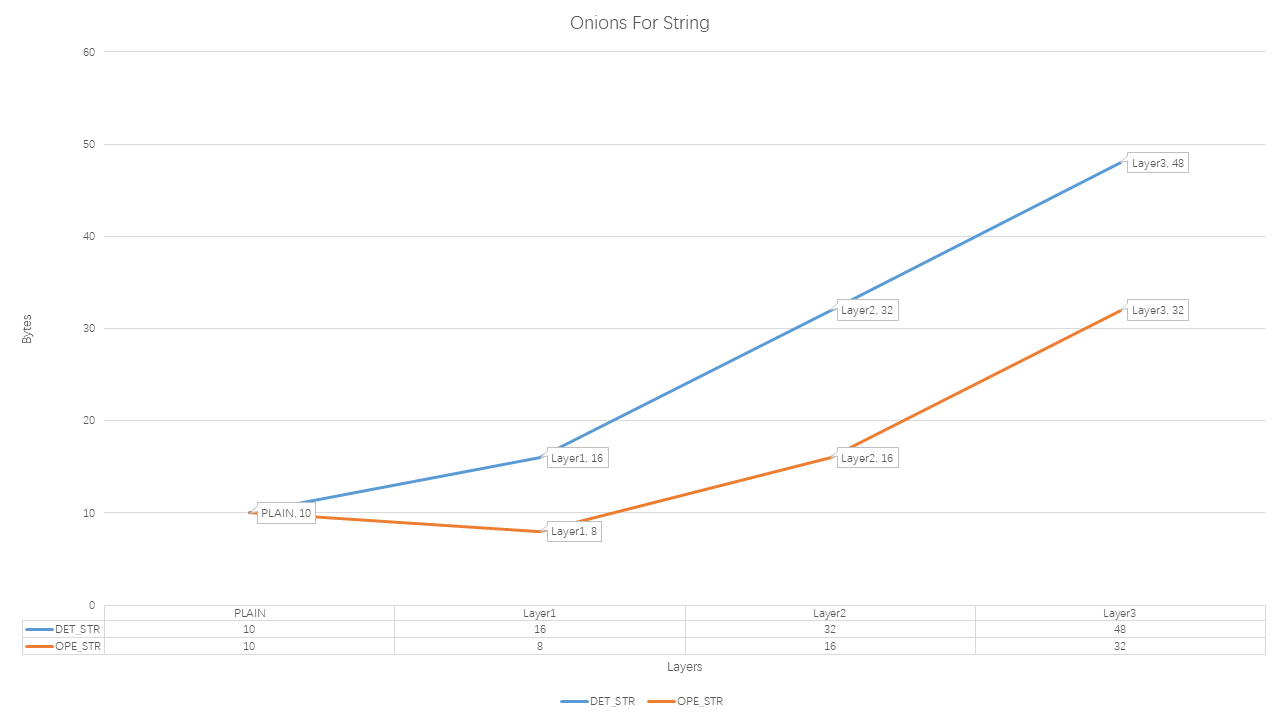
\includegraphics[width=\columnwidth]{images/onions-for-string.png}
\caption{onions-for-string}
\label{fig:stack4}
\end{figure}


\begin{figure}[tb]
\centering
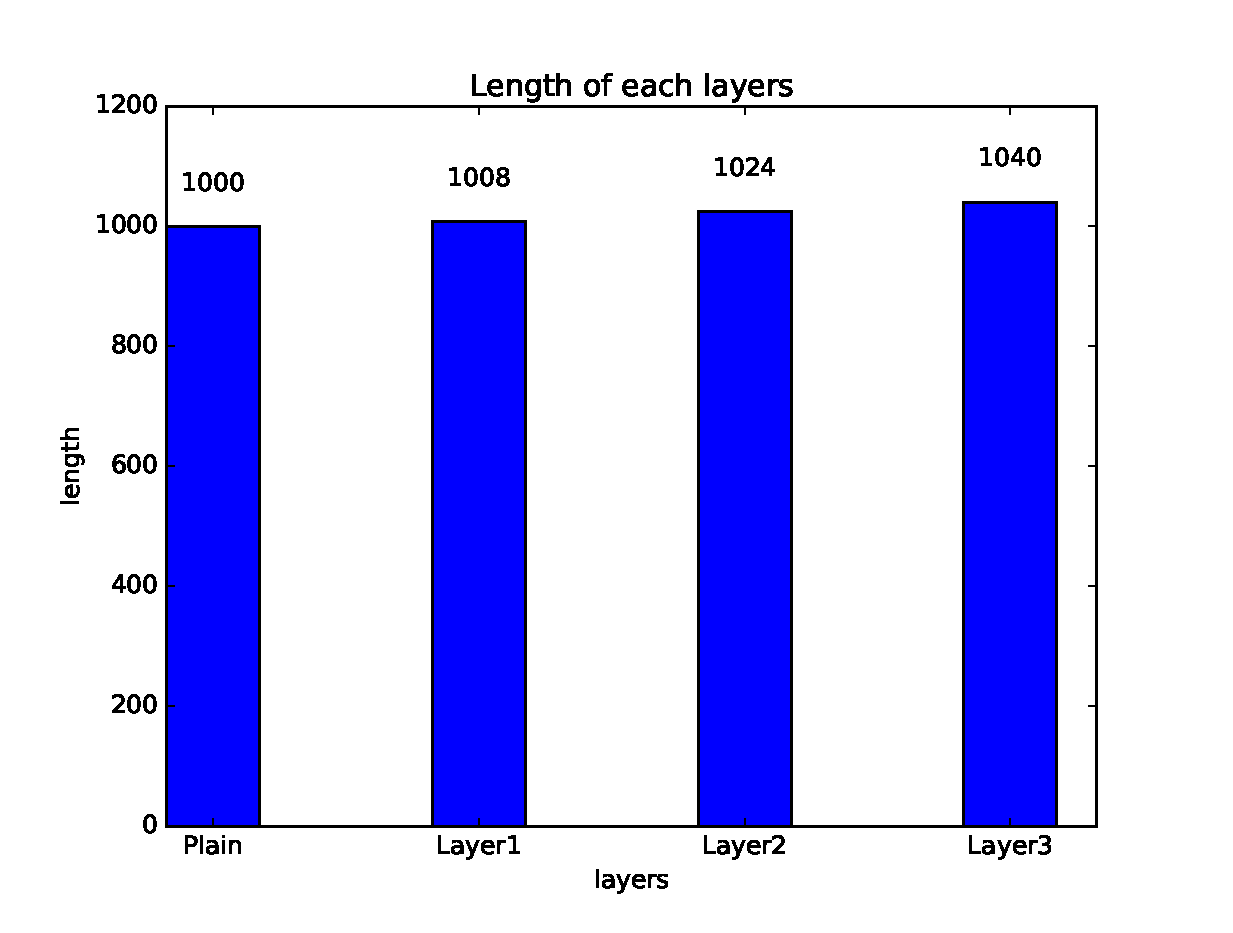
\includegraphics[width=\columnwidth]{images/det_str.eps}
\caption{det-str-eps}
\label{fig:stack5}
\end{figure}



Figure~\ref{fig:stack4},~\ref{fig:stack5} shows how the size of a string change for each onion and each layer of the onions. As the figure depicts, for the onion DET, the plain text is 10 Bytes long, while the size of the onion in layer RND is 48 Bytes long. That because the onion DET has three layers, namely DET-JOIN, DET, and DET-RND. The first two layers uses AES-CMC for encryption, and the third layer uses AES\_CBC. In the current implementation, block size of 16 bytes is uses. In current version of CryptDB, the input text of the algorithm can not be divided exactly by the block size, then the input should be padded with zero to make it divisible. If the input text is divisible, cryptdb will pad the text by one block. So, for plain text with size 10 Bytes, after it is encrypted with layer DET-JOIN, it becomes 16 Bytes. After it is encryptdb with layer DET, it is padded to 32 Bytes. And when it is in layers DET-RND, the size becomes 48 Bytes. Note that for ciphertext, CryptDB used only the integer type of MySQL if the size of ciphertext can fit in that data type. Otherwise, varbinary is used instead. Since Onion Search is not implemented properly, we do not include it in the figure. In fact, the onion search is quiet simple: it has only two layers, and according to \citep{song2000practical}, the size of ciphertext is roughly the same as plaintext. In the current implementation, the change of data type and size of OPE is quiet complex. In fact, the Onion OPE only guarantee the properity of order preserving for 8 bytes prefix of a string.




\begin{figure}[tb]
\centering
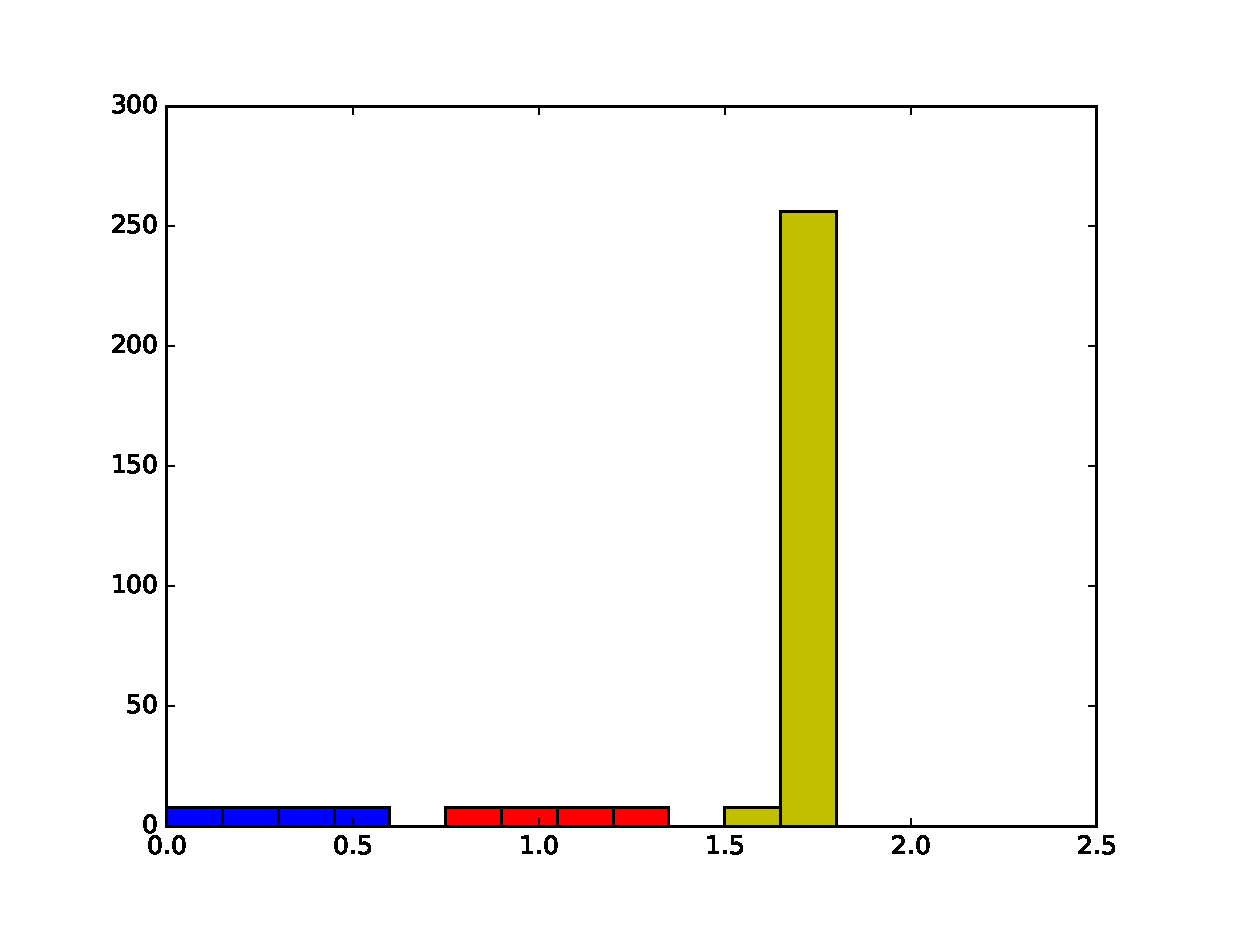
\includegraphics[width=8cm]{images/onion-for-integer.eps}
\caption{onions-for-integer}
\label{fig:stack6}
\end{figure}


Figure~\ref{fig:stack6} shows how the storage size change for each onion for integer type. Currently, there are three onions for integer, HOM uses Pailliar algorithm, DET for integer uses 64bits blowfish, so the size of the ciphertext is always 64bits integer. There is no padding. HOM uses pailliar, so the result is always 256bytes integer. MySQL do not has such long integer, so varbinary(256) is used instead. Now let's discussion how the size change across layers of the onion OPE for both String type and Integer type. 



OPE requires that the cipher text size is double the size of plain text. Let's first discuss OPE-INT. This onion has three layers, namely OPE-INT-JION,OPE-INT,OPE-RND. If the plaintext is of the type tinyint, which has only 1 Bytes. Then after the layer OPE-INT-JOIN, it becomes 2 Bytes, and after the layer OPE-INT, it becomes 4 Bytes. So for the layer OPE-RND, the input is a 4 Bytes long integer, and the result of OPE-RND can be represented by a 8 Bytes bigint in MySQL. If the size of the integer is 64 bits, then after the encryption of one layer of OPE, the ciphertext should be 128 bits, which can not fit in an integer type. Cryptdb uses 128 bits varbinary data type. In that case, the input of the layer rnd is string instead of integer, so algorithm AES is used instead of blowfish. So the onion OPE-INT may contain layer RND-STR. 

Then let's talk about OPE-STR. OPE-STR can also have three layers, OPE-STR-JOIN, OPE-STR, OPE-RND. When the input of the algorithm is a string, plaintext length of 4 Bytes and  ciphertext length of 8 Bytes are specified. That is, only the prefix are encrypted and has the properity of order preserving. Then in the layer OPE-STR, since in the first layer, the data type has been transformed to 64bits integer, the OPE-STR is transformed to OPE-INT, and the input is 64bits long. So after this layer, integer can no longer fit ciphertext. The data type has become 128 bits varbinary type. And then in the third layer, aes is used for the layer, adding one block to the size, making the total size of the onion 32 Bytes.


The above discussion reveals two facts:

\begin{itemize}
\item[--] The size of Onion OPE can not exceed 32 Bytes regardless of the size of plaintext
\item[--] Onion OPE can loose information of the plaintext, so we can not use the Onion OPE
\end{itemize}



As we have known the property of the encryption schemes and the data layout. We can now start to design the strategy of deduplication. We will first discuss each onion and then give three simple strategies for analysis. Then in the experiment section, we will use our workload to test the strategies. We first discuss the design choices for each onion of interger data and string data. 


\begin{itemize}
\item Integer/String OPE: For ope-int, we have little choices, since OPE is not able to be decrypted. If this onion is removed, then we need two OPE-Encrypt operation and one AES-enctypt operation to get it back. 
\item Integer HOM: HOM takes a long time to recover, and also occupy 256 Bytes. If we choose to remove it, we should use one Paillar-encrypt operation to get it back. Only retaining HOM is never a good choice, because it takes a long time to decrypt HOM for recovery, and also the storage size is large. So HOM should be removed or be retained together with other onions.
\item Integer/String DET: If this onion is removed, then it takes three blowfish-encrypt operations to recover it. For String type, we need two AES-CMC-encrypt and one AES-CBC-encrypt operation to recover the onion. The encryption time is related to the size of the string.
\item Integer IV: 8Bytes integer. faster to regenerate
\end{itemize}



Since the detailed performance is related to so many things, we do not provide exact strategy for backup. Instead, we summarize several Principals for cryptdb backup and then give some examples. 

\begin{itemize}
\item[--] One original field is replicated several times and encrypted with different schemes
\item[--] If we want mininum storage overhead, then for each field we can find the onion with the least size, like AES or blowfish, that can produce ciphertext of the size similar to plaintext, and remove all other onions. If we want minimum time overhead, we should backup all the onions, so that we can recover the data directly. Other choices are something in between.
\item[--] Metadata should have a full backup for data recovery, and the size of metadata is small. 
\item[--] For recovery, we need to decrypt the onion we have, and based on the metadata, recompute the ciphertext for other onions.
\item[--] For one onion, we can choose the stay in RND layers, which means identical plaintext can have different ciphertext. If we decypt it to a layer that is not random, then identical plaintext can have the same ciphertext. If most of the plain text in this column are the same, then it will be easy to compress this filed to reduce storage overhead. Also, if we decrypt RND layer, then we can remove the IV column, which further reduces storage overhead.
\end{itemize}


Based on the principals, we proposes the following strategies for String data and Integer data. 

\begin{itemize}
\item[--] Remove RND and use DET onion will produce the least storage overhead.
\item[--] Do not remove anything. This is the strategy with the most storage over head and least computation overhead
\item[--] Retain RND and salt for DET, remove HOM and OPE, and Search. This method has high security level.
\end{itemize}




For those two data types and strategy, we construct microbenchmark to do experiments. Actually, the time needed for recovery can be reduced by using multi-threading or other optimization. We assumes that other factors are the same and only condiser the overhead of recomputation. We use single thead whith pipeline insert.

So, the overall strategy looks like the following: we let users choose the strategy bases on the what they care about. They can either choose to backup all the onions, or choose to have minimum backup or something in between. Figure~\ref{fig:stack7} and Figure~\ref{fig:stack8} shows how to encrypt and extend the plain text, and then choose one onion for back up, and then compress the onion. For recovery, we should first decrypt the onions and then recompute the deleted onion. Then we should be able to construct the sql queris for recovery. This is the same as the logical backup recovery method.

\begin{figure}[tb]
\centering
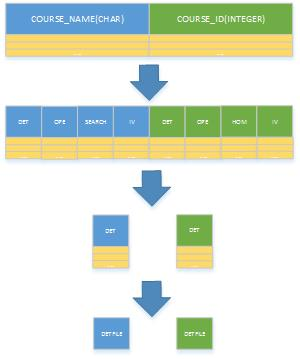
\includegraphics[width=4cm]{images/Workflow.jpg}
\caption{Backup and compression}
\label{fig:stack7}
\end{figure}


\begin{figure}[tb]
\centering
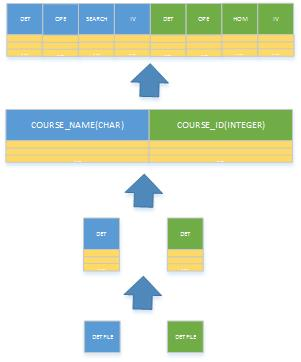
\includegraphics[width=4cm]{images/Recovery.jpg}
\caption{Aes encryption and decryption time}
\label{fig:stack8}
\end{figure}


\section{Evaluation}

Our experiments are performed on a machine with Intel(R) Xeon (R) CPU E565 2.4GHz in Ubuntu 16.04. 


There are two things to evaluate, the first is the storage overhead, and the second is the time consumed for recovery. It should be noted that storage overhead for logical back up is not the same as the storage overhead in the DBMS since they use different data representation. For example, 64 bits integer should occupy 64 bits in the DBMS, However, in logical backup, integer is stored as string, which means the storage overhead is related to the length of the string. For example, the integer 123456789 can occupy 72 bits. In our evaluation, we compute the storage overhead based on the string representation as the logical backup tool mysqldump do. For time consumpation, we choose to first evaluate each kind of encryption algorithms and then give the estimated time overhead for recovery. We do not evaluate the total time consumpation for recovery since different logical backup tools can have different recovery speed, this speed is influenced by implementation optimizations like multi-threading or batch insert, which are not related to our topic. So we only estimate the time for recovering to the logical representation of the data. 


First, we analyze the overhead of time.  Recall that we may want to remove salt, so we first need to know how fast can we regenerate a new salt. We do experiment with the function in CryptDB and find that the computation overhead for one salt value is around 0.7 $\mu$s. So this computation is quite fast and the overhead could be ignored. We also need to know how much time is consumed to do computation in each layer, so we do experiment for those algorithms.


\begin{figure}   
  \begin{minipage}[t]{0.5\linewidth}  
    \centering   
    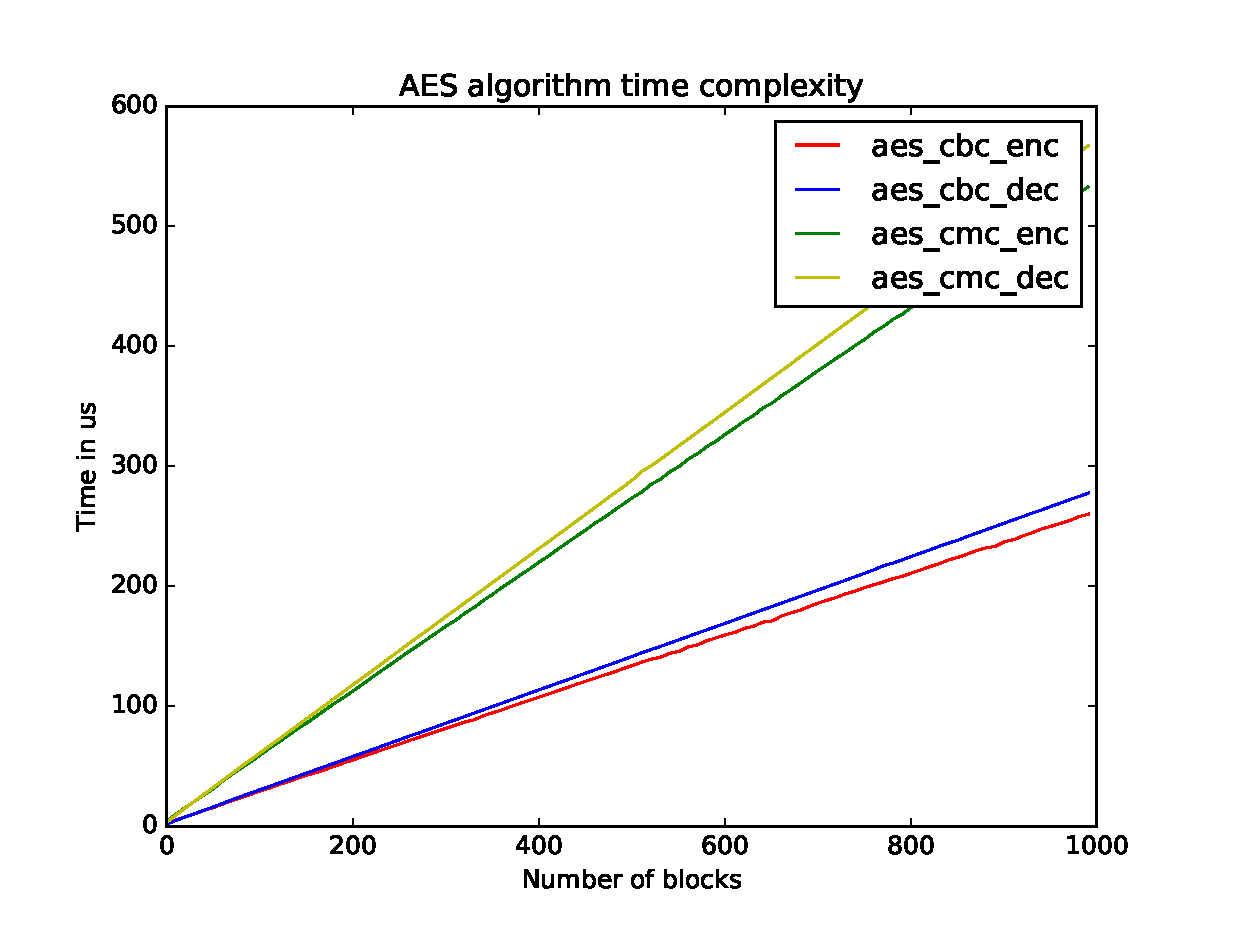
\includegraphics[width=4.0cm]{images/aes.eps}   
    \caption{This figure show how the encryption and decryption time change with the input length.}   
    \label{fig:stack9}   
  \end{minipage}%   
  \begin{minipage}[t]{0.5\linewidth}   
    \centering   
    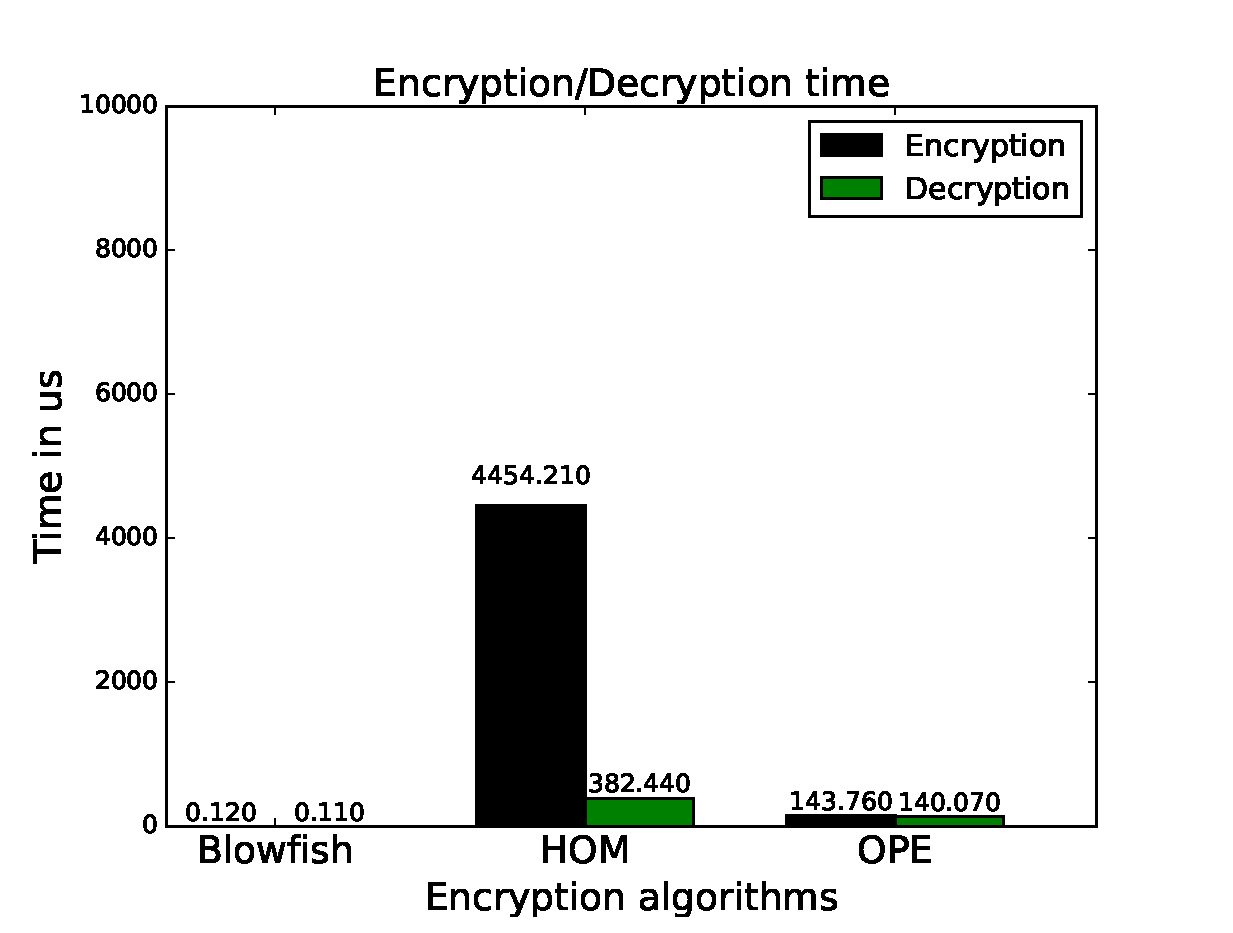
\includegraphics[width=4.0cm]{images/time.eps}   
    \caption{This figures show the encryption and decryption time of the algorithm blowfish, Pailliar, and order preserving encryption}   
    \label{fig:stack10}   
  \end{minipage}   
\end{figure}

% \begin{figure}[tb]
% \centering
% 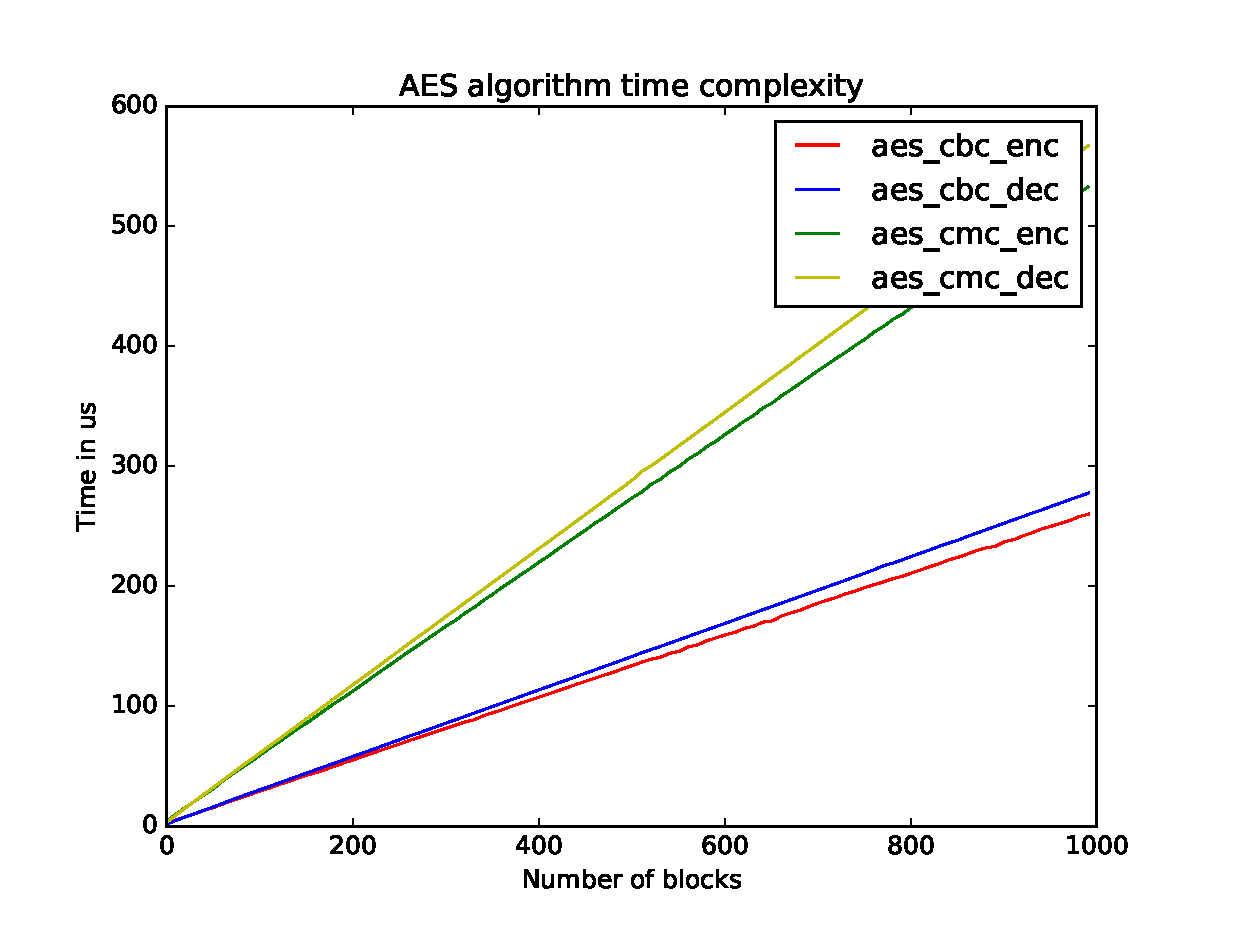
\includegraphics[width=8cm]{images/aes.eps}
% \caption{Aes time consumpation}
% \label{fig:stack9}
% \end{figure}




% \begin{figure}[tb]
% \centering
% 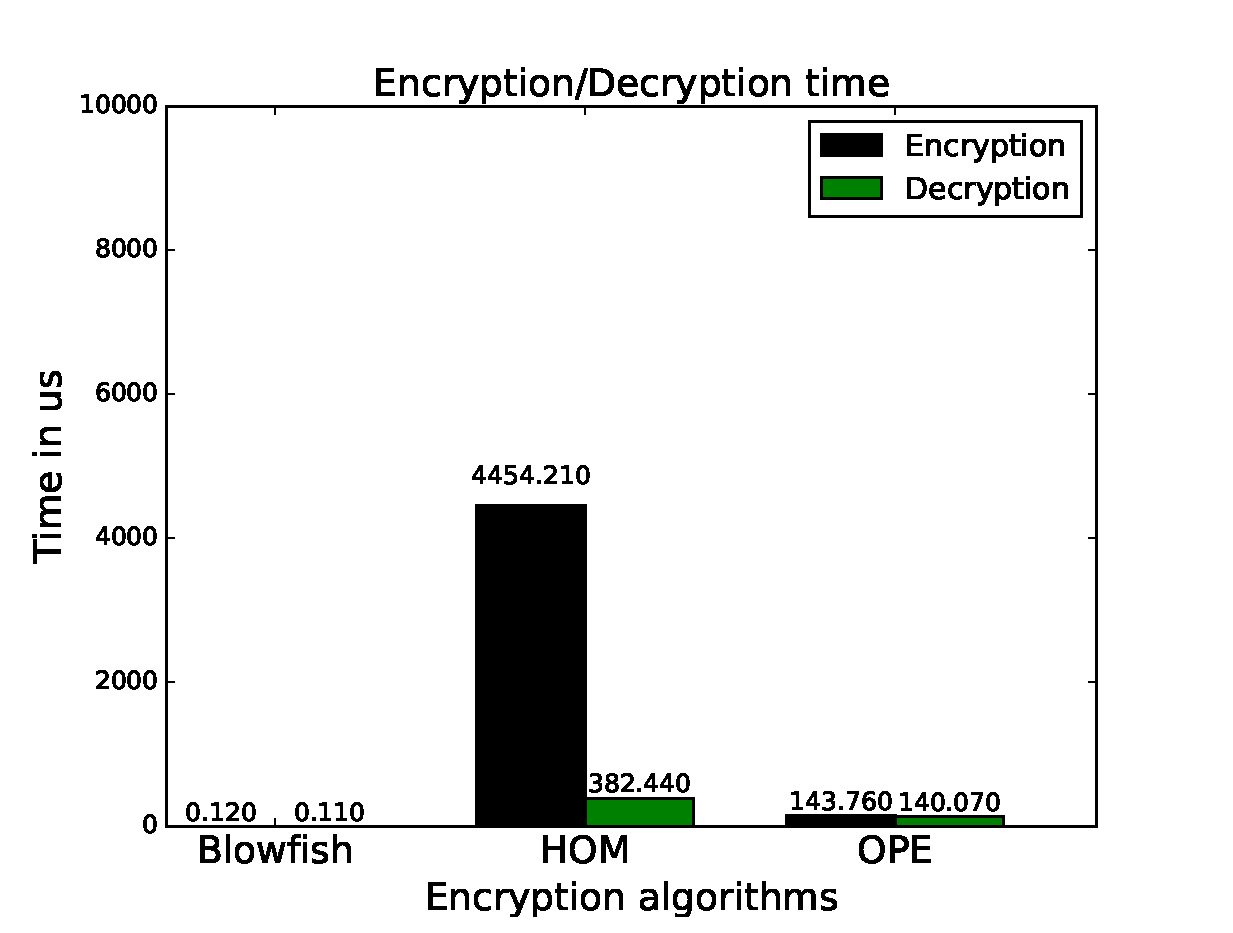
\includegraphics[width=8cm]{images/time.eps}
% \caption{time consumpation}
% \label{fig:stack10}
% \end{figure}


Figure~\ref{fig:stack9} shows the time consumption for encryption and decryption for AES-CBC and AES-CMC. AES-CBC is a simple wrapper of AES function in the open-ssl library, and AES-CMC is a wrapper of AES-CBC  which internally calls AES-CBC twice. So the time for encryption and decryption of AES-CMC is roughly twice that of AES-CBC, and the time consumption is almost proportional to the size of plaintext. Figure~\ref{fig:stack10} shows the encryption and decryption time for pailliar, blowfish, and the order preserving encryption. We can find that blowfish, which operate on 64 bits integer, is fast. OPE is also fast. HOM, which uses pailliar, is slow. 9.1ms is used for encryption, which means the throughput of inserting one column of integer is limited to around 100 rows per second.

We now begin to analyze the two type of data that is supported by CryptdDB. We create one simple table with only one field, and backup that encrypted data, and show the size of each encrypted onion. Note that this is not exactly the same as logical backup since in logical back, data is in the form of sql queries. We do not backup the data in SQL query form because the logically deduplicated queries, which are not complete, can not execute on the DBMS directly. So we choose to backup each column separately, something like the 'SELECT into file' method.

For integer data, as we mentioned before, the columns are replicated three time for three onions with an additional salt column for the decrypting the layer RND. We insert 1,000,000 integers, all of them are simple 12345. Figure~\ref{fig:stack11} shows the size of each onion when backed up. We dump each column into separate files and use 'du -h' to find the size of each column when in string representation. We can find that HOM is the biggest, since it's data type: varbinary(256), when in string representation, occupies large space. IV is random 64 bits integer, DET is also random 64 bits integer, so they are of similar size. OPE is larger than DET, since the type is varbinary(32) in rnd layer. 


% \begin{figure}[tb]
% \centering
% 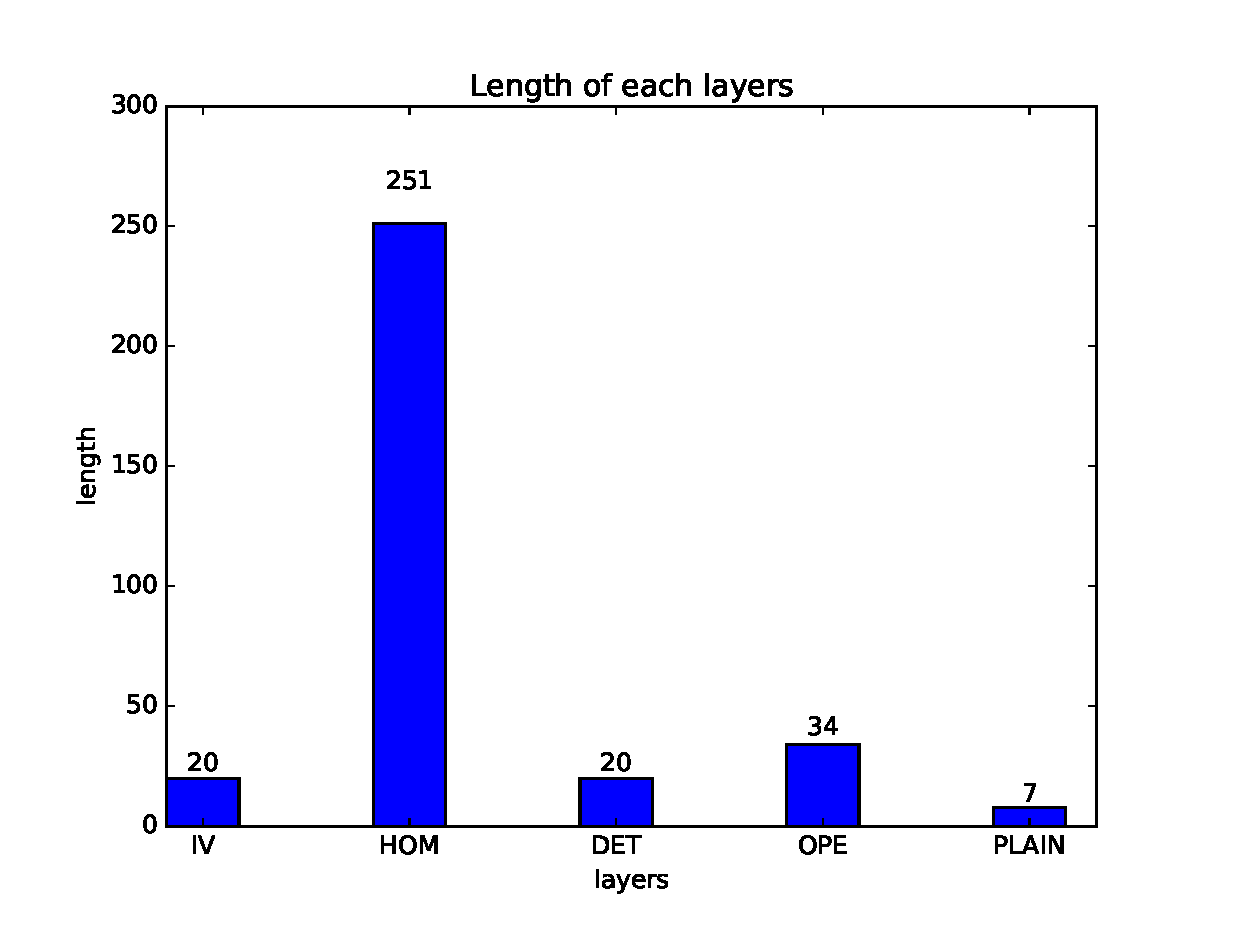
\includegraphics[width=8cm]{images/size-of-each-onion.eps}
% \caption{Size of onion for integer type}
% \label{fig:stack11}
% \end{figure}



\begin{figure}   
  \begin{minipage}[t]{0.5\linewidth}  
    \centering   
    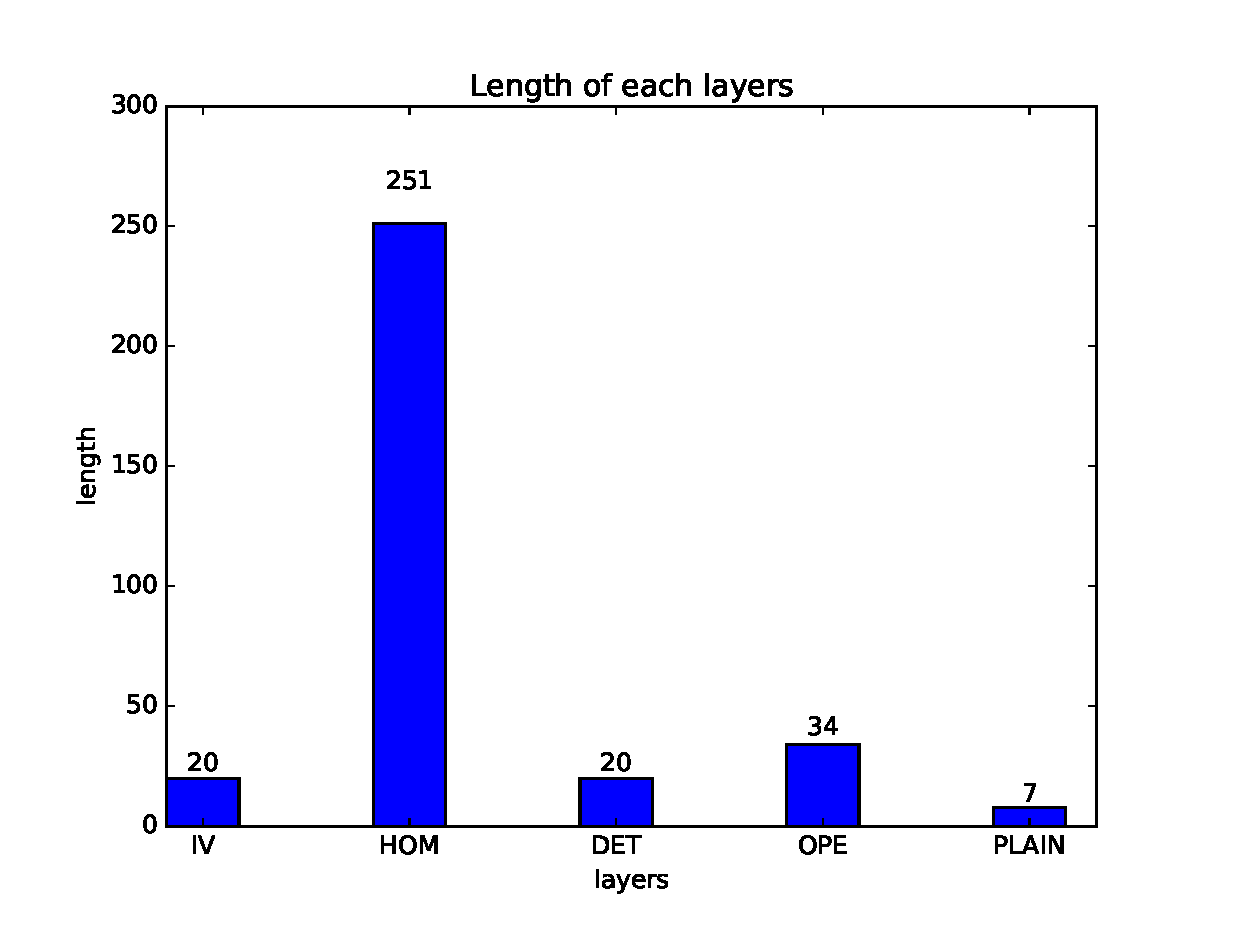
\includegraphics[width=4.0cm]{images/size-of-each-onion.eps}   
    \caption{This figure shows the size of each encrypted column in the form of text file for the table we creates that has one plaintext column of Integer type}   
    \label{fig:side:a}   
  \end{minipage}%   
  \begin{minipage}[t]{0.5\linewidth}   
    \centering   
    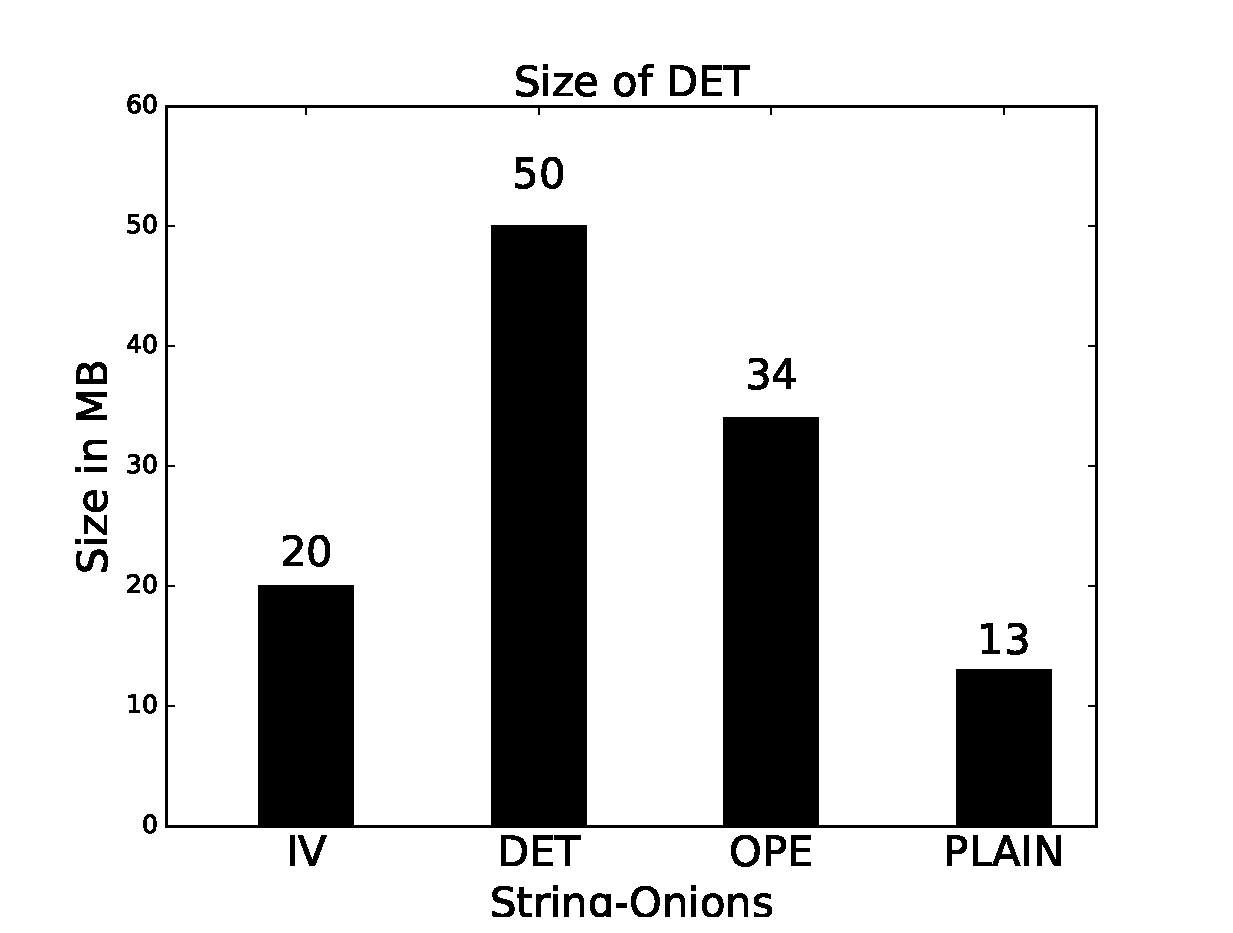
\includegraphics[width=4.0cm]{images/det-rnd.eps}   
    \caption{This figure shows the size of each encrypted column in the form of text file for the table we creates that have one plaintext column of String type}   
    \label{fig:side:b}   
  \end{minipage}   
\end{figure}





For string type, we do experiment with a simple table of varchar(10). After encryption, the onion DET will be tranformed to varbinary(48) due to the padding, and OPE will be varbinary(32), salt should be big int. We insert 1,000,000 plaintext of length 10 into the table, and the Figure~\ref{fig:stack12} depicts the results for each column.We can find that even for very short string, three layer of encryption in onion DET can make it larger than the onion OPE. So ope is always assumed  smaller than DET. And the size of salt remains the same as in the experiment with integers. We can find that decrypting the RND layer can produce greater compression ratio. We use gizp with default options. This is an extream case since all the data in the columns are the same. For a big column with low Cardinality, like gender, this approach is expected to produce similar results. 


% \begin{figure}[tb]
% \centering
% 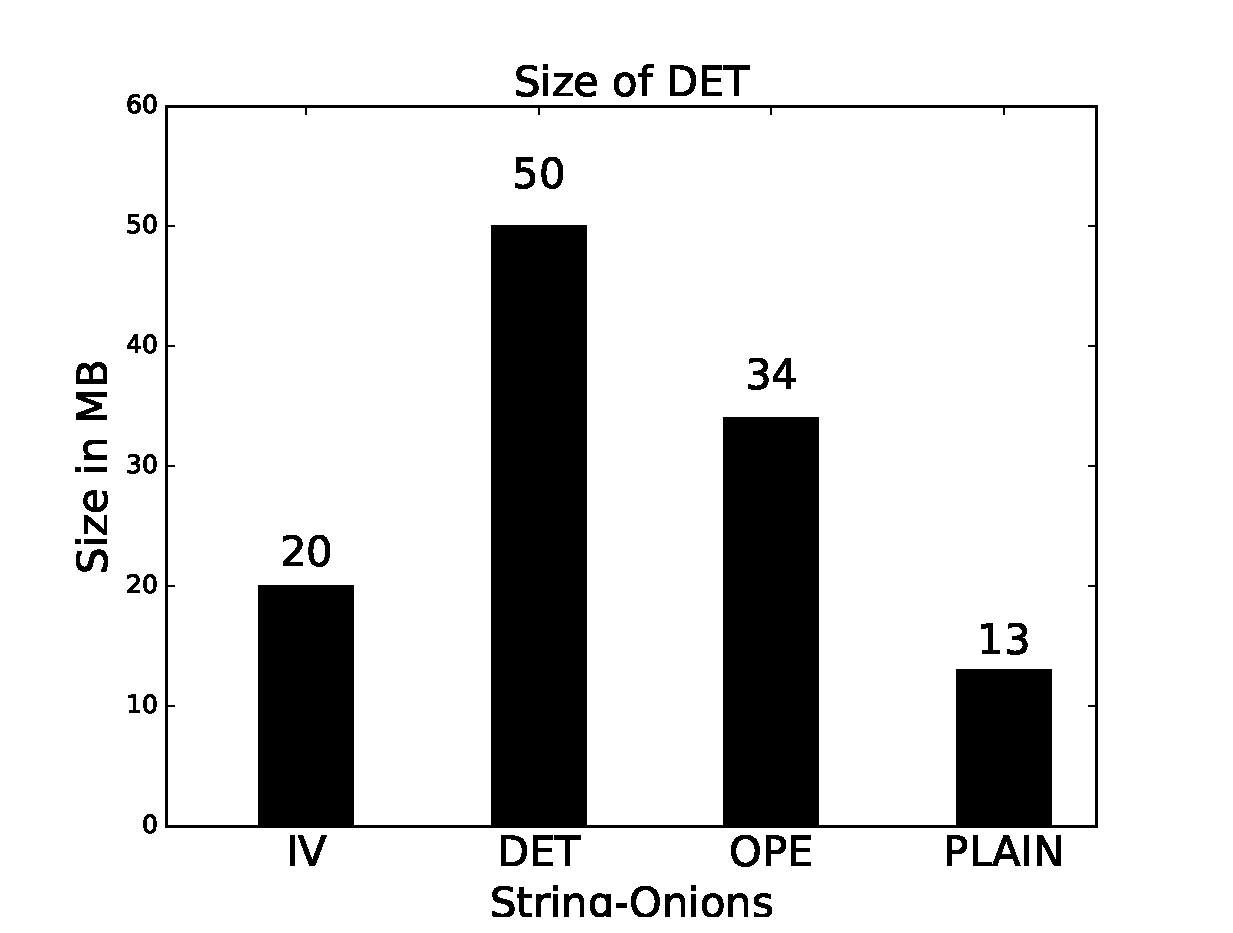
\includegraphics[width=8cm]{images/det-rnd.eps}
% \caption{size of onion for string type}
% \label{fig:stack12}
% \end{figure}



\begin{figure}   
  \begin{minipage}[t]{0.5\linewidth}  
    \centering   
    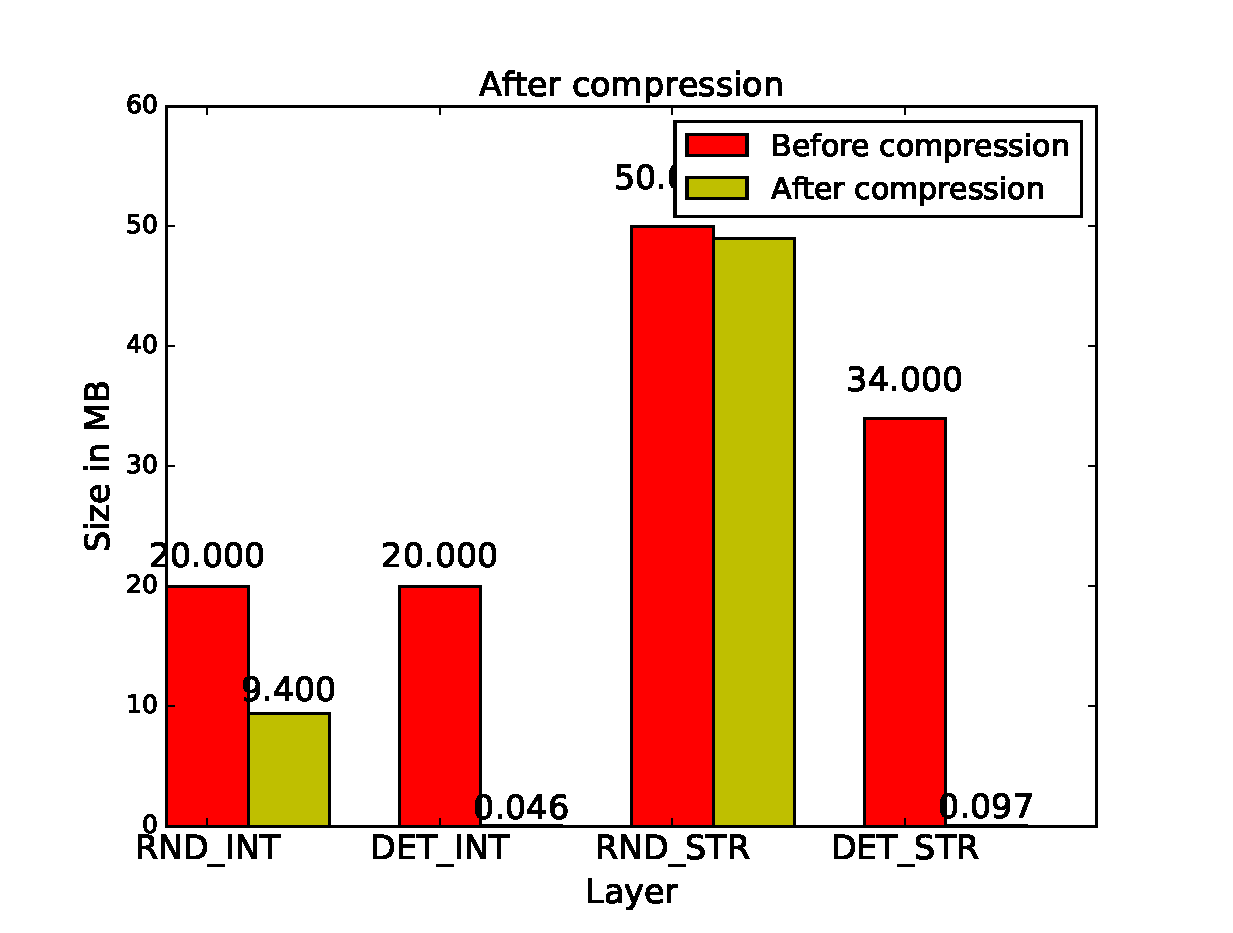
\includegraphics[width=4.0cm]{images/aftercompression.eps}   
    \caption{This figure shows how the size of each encrypted column change after being compressed using gzip}   
    \label{fig:side:a}   
  \end{minipage}%   
  % \begin{minipage}[t]{0.5\linewidth}   
  %   \centering   
  %   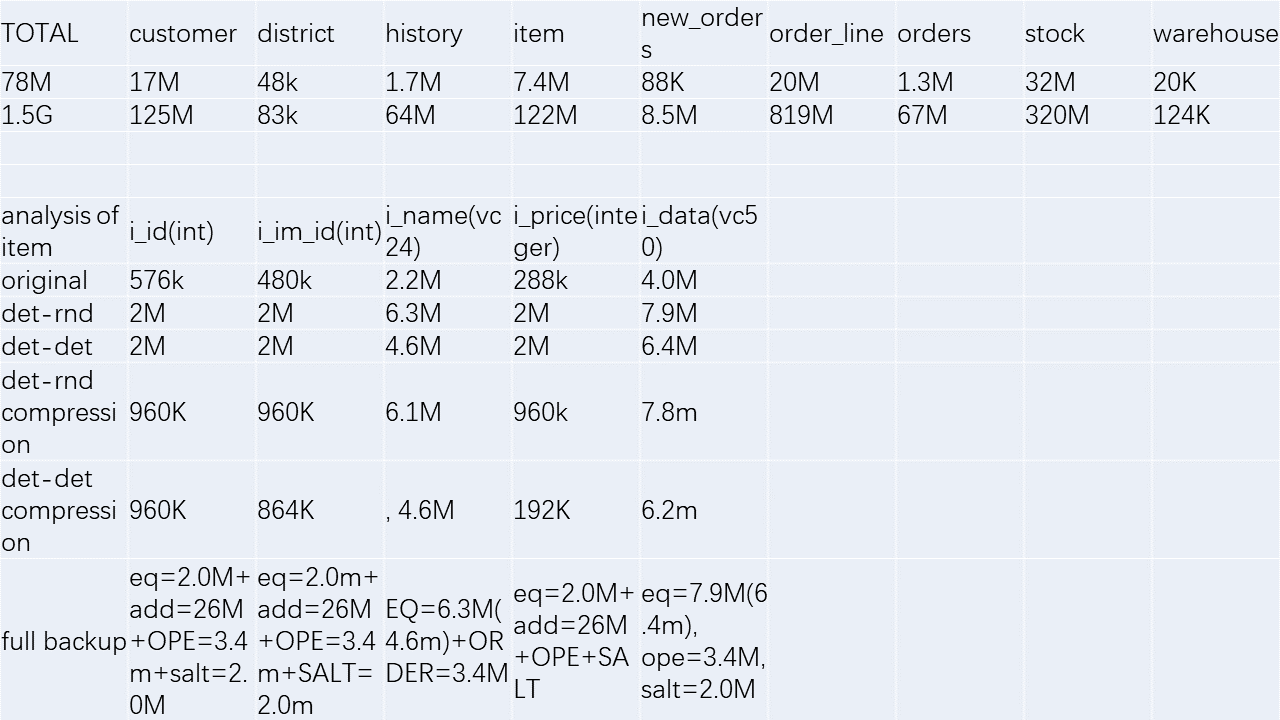
\includegraphics[width=4.0cm]{images/tpcc.png}   
  %   \caption{tpcc}   
  %   \label{fig:side:b}   
  % \end{minipage}   
\end{figure}



% \begin{figure}[tb]
% \centering
% 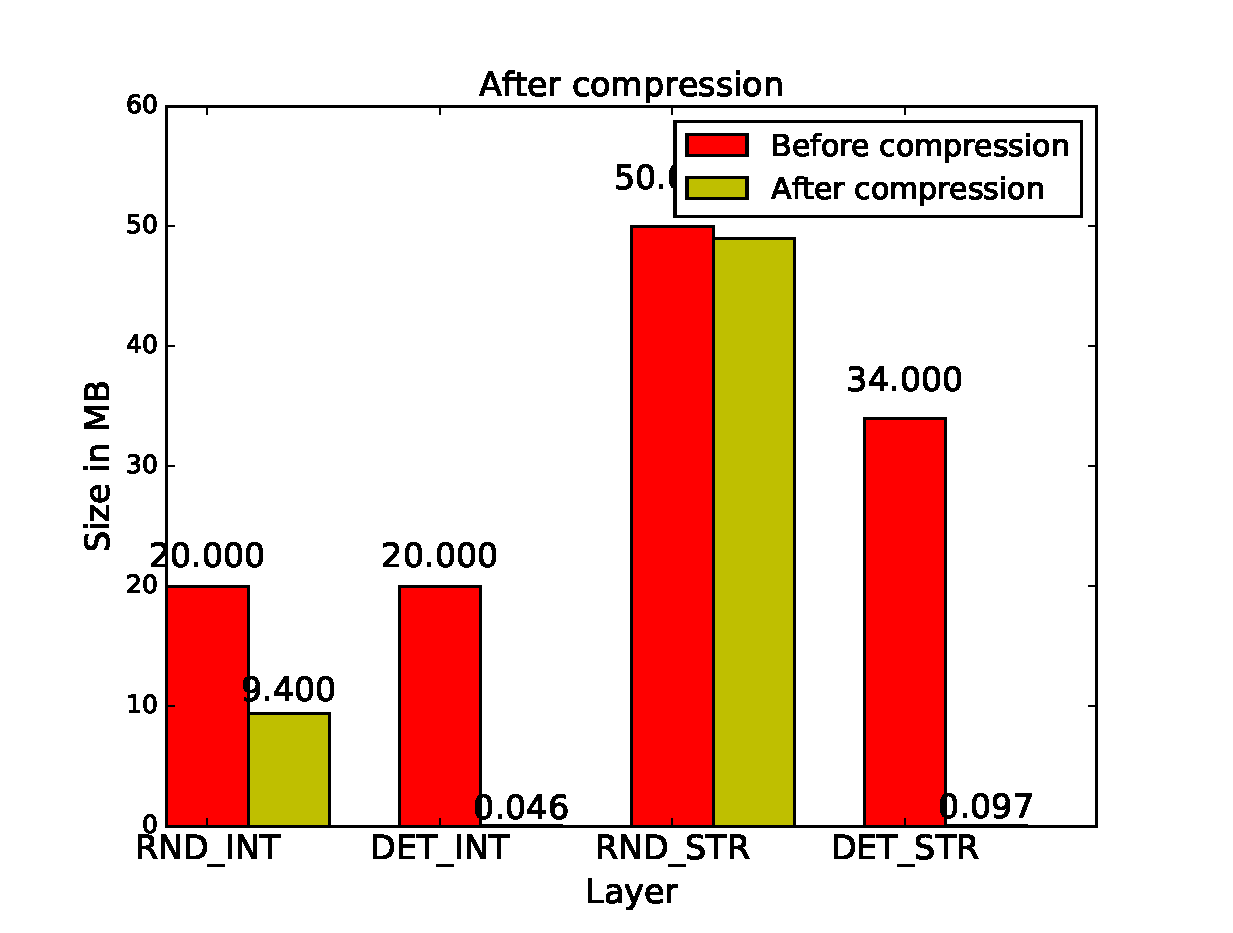
\includegraphics[width=8cm]{images/aftercompression.eps}
% \caption{size of onion for string type}
% \label{fig:stack12}
% \end{figure}


We also give the expected recovery time for each onion based on the assumpation that we only backup the Onion DET. Figure~\ref{fig:stack12} depicts the results.


Finally we do experiment with the TPCC-MySQL, the original data is the 74MB, and the encrypted data is 1.5 GB. So there is large expansion. especially for those tables that has columns of integers of small value like 0,1. Those could be stored with 1 Bytes should now pay the 256 Bytes overhead of the onion HOM, inaddition to other onions and the IV column. We can use the simplest method to backup only the DET and IV column, which is 229M+125M. 
% Figure~\ref{fig:stack13} depicts the results. As we have mentioned, analyzing a table can be easy since the characteristics of each column is known. 


% \begin{figure}[tb]
% \centering
% 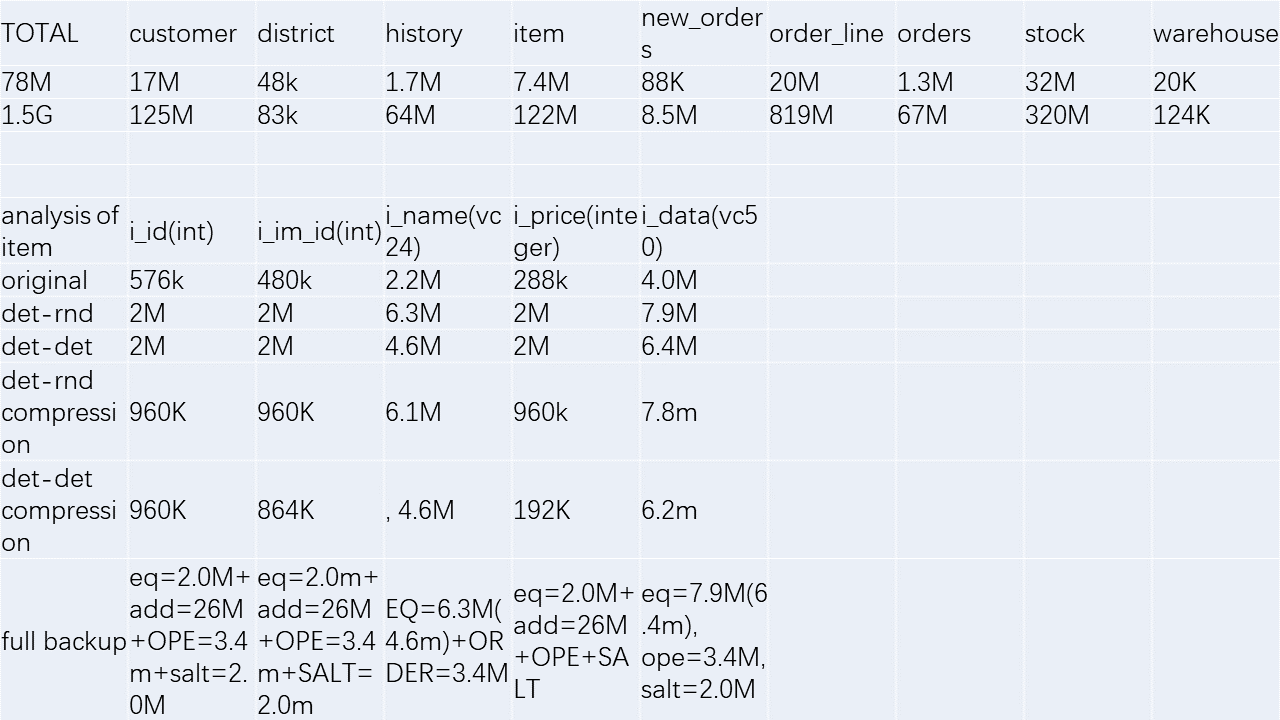
\includegraphics[width=8cm]{images/tpcc.png}
% \caption{tpcc data}
% \label{fig:stack13}
% \end{figure}





Based on the above results, we can find that, in the current implementation of CryptDB, Onion OPE is always small and can not be used for recovering, So OPE can be removed  to save space. For integers, the onion HOM is large, and also taken a long time to recover, So If we remove HOM for deduplication, and use the onion DET for recovering the data, we can save a lot space while paying the overhead of recomputing the onion HOM. If we can find ways to accelerate the computation of pailliar, then this deduplication can be more efficient. The onion DET-INT uses blowfish, which is fast and occupy little space compared to the plaintext, so it's reasonable to retain this onion. Decrypting the layer RND-int should reduce the size by half since we no longer need the IV column, so we can remove this column. Also, decrypting the RND-int layers can produce higher compression ratio. Things are similar for string type. String type has a search onion, which is expected to be similar to onion DET. So if we remove search, we expect to reduce the size by half. If we then remove the RND-STR layer, we also get higher compression ratio. In \citep{popa2015guidelines}, new onions are added in CryptDB, this can leave more space for deduplication.


% \begin{talbe*}
% \begin{tabu*} to \hsize {|X|X|X|X|X|X|X|X|X|X|}
% \hline
% Tablename & customer & district & history& item & new\_order & order\_line& orders & stock & warehouse \\ \hline
% DET & 1 & 2 & 3& 1 & 2 & 3& 1 & 2 & 3 \\ \hline
% OPE & 1 & 2 & 3& 1 & 2 & 3& 1 & 2 & 3\\ \hline
% HOM & 1 & 2 & 3& 1 & 2 & 3& 1 & 2 & 3 \\ \hline
% IV & 1 & 2 & 3 & 1 & 2 & 3& 1 & 2 & 3\\ \hline
% TOTAL & 1 & 2 & 3 & 1 & 2 & 3& 1 & 2 & 3\\ \hline
% \end{tabu*}
% \end{table*}

% % \begin{talbe*}
% \begin{tabular}{ccc}
% \toprule
% 2&9&4\\
% \midrule
% 7&5&3\\
% 6&1&8\\
% \bottomrule
% \end{tabular}
% % \end{table*}



% \begin{table*}
% \renewcommand{\arraystretch}{1.3}
% \label{tab:example}
% \centering
% \begin{tabular}{|c|c|c|c|c|c|c|c|c|c|c|}
%   \hline
%   % after \\: \hline or \cline{col1-col2} \cline{col3-col4} ...
% &total & customer & district & history & item & new\_order & order\_line & orders & stock & warehouse   \\
% DET &  & 13M+9M+5.1M+3.8M+9*608K & 1 & 1 & 1 & 1 & 1 & 1 & 1&1 \\  
% OPE &  & 13*976k+8*608k & 1 & 1 & 1 & 1 & 1 & 1 & 1&1 \\
% HOM &  & 7.4M*9 & 1 & 1 & 1 & 1 & 1 & 1 & 1&1 \\
% IV &  & 608k*21 & 1 & 1 & 1 & 1 & 1 & 1 & 1&1 \\
% \hline
% \end{tabular}
% \caption{This table shows the size of each of tcpp-mysql's table's onions and IV column}
% \end{table*}
\section{implementation}

In this section, we describe briefly the problems we meet while doing experiments and the method we use the tackle those problems. The neweset version of cryptdb do not support STMT\citep{mysql-stmt} queries, and TPCC-MySQL uses STME to load data. We do not currently implement STMT for cryptdb, instead, we first insert plaintext data into cryptdb, dump data into a .sql file , and then insert data into cryptdb using this file to avoid using STMT. The tool mysqldump has default option of extended-insert\citep{mysqldump-extended-insert}, but if the size of insert query exceed a certain length, cryptdb can not support it. So we reconstruct the data to limit the size of extended insert. We only use warehousre two, and modify the data type of the tables that is not supported by cryptdb. Namely, we change date type to string type, float to integer type, signed integer to unsigned integer type. TPCC is the standard benchmark, so we still want to show the resutls based on it. The detailed configuration is aviliable at this site\citep{practical-cryptdb}.

For the backup choices, we should parse the metadata structure of cryptdb. For example, having the database name and table name, we should know such information as how many fields does the table have, how each field is replicated and encrypted, and the encrypted field name of each onion. All those information are stored in the database in the proxy, and can be parsed by reading the data and parsing the data. Those functions can be implemented in less than 800 lines of C++ Code, including the testing code. Our future work should make cryptdb stable and add new features to it, the backup code can also change due to that kind of change, but the underlining principal for backup is universal. To remove the layer rnd, we currently can only mannualy issue queries to cryptdb and then use the onion adjustment function to  accomplish that.

Current version of cryptdb also remove the layer ope-jion, we implemented it in our version of cryptdb and so the onion ope has three layers. The modified version and the related code are available at \citep{practical-cryptdb}.

\section{related work}

% We propose high level deduplication technique the used the metadata in the proxy to find fields in a relational table that are duplicated and encrypted using different encryption schemes. We find proper fields to remove and save the deduplicated field into files. Our technique can be considered as a kind of preprocessing and can be combinded with other deduplication methods.


\textbf{backup, dedpulication, and compression} Based on the format of backup, database backup can be categorized into two types: logical backup and physical backup\citep{mysqlbackup}. Our deduplication technique find sementically identically columns of a encrypted table, and backup one copy of the column into text file, which is a kind of logical backup. 

% Deduplication on storage system is a hot research topic\citep{paulo2014survey}.

According to \citep{mandagere2008demystifying}, compress tools like gzip reduce intra-file duplication while deduplication reduces both inter and intra file deduplication. 
% They do not address the problem of encrypted database. 
Those deduplication can be categorized into three types: file level, block level, and byte level deduplication. Those dedup systems are unable to find duplicate columns in cryptdb backup workload since data are encrypted using different encryption schemes.\citep{xu2017online} proposes an online deduplication for operational database system while our work focus on backup workload.

% According to \citep{xu2017online}, dedup using hash method works well for both primary and backup storage data sets that comprises of large files that are rarely modified. In our work, we focus on archivial data, so the files are rarely modified. 

% And those traditional method can work together with our proposed method. There are many work on deduplication for secondary storage, the can either use exact dedup\citep{dubnicki2009hydrastor} or similarity based dedup\citep{xu2015reducing} \citep{aronovich2009design}\citep{you2005deep}. 


 % Actually, block level comparision do not work well for database workload, so there are also research targeting database workload. 

% These traditional chunk based dedup system can not handled encryption well, So there are also work that address the tension between encryption and deduplication.

% For backup database that is encrypted, they can not find duplicates since data are encrypted. 
% In our work, we can first use metadata to find duplicate data that is encrypted using different encryption schemes, and backup only one copy of the data. Then the backup can be fed into traditional deduplication or compression systems. We also find that removing the onion layer RND provides the potentail for greater compression ratio. 

\textbf{encryption and deduplication} Data in Cryptedb is encrypted, and encryption and deduplication are in tension, and there are researches about this issue.\citep{bellare2013message} \citep{puzio2015perfectdedup} proposed message-locked enctyption, a kind of convergent encryption to addressed this problem. They require that data is encrypted using the proposed scheme, while in cryptdb, the encryption scheme is fixed, so those work do not target on cryptdb. \citep{yan2016deduplication} addressed the problem of deduplication of encrypted files in a multi-user situation through authorized party and token comparison, they proposed their strategy through ownership chanllenge and proxy-re-encryption. Those work do not target on database backup, and our work target on encrypted database that is replicated to support computing on encrypted data.


% In constrast, our work forcus on generating a backup file that occupy less storage space. In fact, deduplication methods on encrypted data fall into two catagories, convergent encryption and proof of ownership\citep{akhila2016study}. Convergent encryption works like DET, So detjoin level have the potential to allow deduplication.

% How to combine those two methods together to make efficient deduplication is future work.



% \citep{francinasurvey} proposed three encryption schemes for deduplication, those are file level deduplication.
% There are also work on solving the problem of compression and encryption\citep{zheng2017minicrypt}.


% It also talked about client side deduplication using metadata.



\section{future work}

\begin{itemize}
\item[--] More efficient homomorphic encryption algorithms other than pailliar
\item[--] Deduplication for master-slave replication
\item[--] Deduplication for distributed database
\end{itemize}



\section{Conclusions}

Fully Homomorphic encryption is still not applicable, So researchers proposed encryption schemes that can support only a small set of operations on encrypted data, and use replication to support many operations at the same time. This idea make homomorphic operation possible in database system. In this paper, we found the problem of storage overhead of such kind of systems, and We study Cryptdb, and propose a backup technique that can utilize metadata to find duplicates in encrypted data. We analysed the details of cryptdb, figured out how to use metadata information to find duplicates in the data. Then we analysed the time and storage overhead of the multi-onion structure, and together with this information, we designed a simple strategy that can reduce storage overhead while incurring little time overhead. We implemented a database backup tool for Cryptedb and experiments showed that our tool can reduce storage overhead without exposing plaintext to administors. We also analysed the tradeoff we can make while making a backup.

For Cryptdb, the metadata stored in a local database in the proxy also need to be backed up. For metadata, the owener of data should get hold of it sinced it stores the encryption keys. The proxy can provide information the the server for save back so that data do not get lost, for recovery, this dump should be give to the proxy for reencryption and recovery.


In our system, we use statics collected, such as time consumpation for encryption and decryption, to help make decisions. Those information can change with systems. So beform doing a backup, we can first run test to fetch such kind of information and then backup the data.

Also, our design allow user to choose from a set of space security and space overhead. We can actually remove rnd for deduplication and compression, which make our system compitable to compression systems.

We can also make conclusions of several encryption algorithms.


\begin{acks}
  The authors would like to everyone for their help, without which this work would not have been possible. 
\end{acks}

\bibliographystyle{ACM-Reference-Format}
\bibliography{acmart}
 

\end{document}
